\chapter*{Abstract}

\begin{adjustwidth}{30pt}{30pt}

    In remote sensing, Land Use/Land Cover (LULC) maps constitute important
    assets for various applications, promoting environmental sustainability
    and good resource management. Although, their production continues to be a
    challenging task.  There are various factors that contribute towards the
    difficulty of generating accurate, timely updated LULC maps, both via
    automatic or photo-interpreted LULC mapping. Data preprocessing, being a
    crucial step for any Machine Learning task, is particularly important in
    the remote sensing domain due to the overwhelming amount of raw, unlabeled
    data continuously gathered from multiple remote sensing missions. However
    a significant part of the state-of-the-art focuses on scenarios with full
    access to labeled training data with relatively balanced class
    distributions. This thesis focuses on the challenges found in automatic
    LULC classification tasks, specifically in data preprocessing tasks.  We
    focus on the development of novel Active Learning (AL) and imbalanced
    learning techniques, to improve ML performance in situations with limited
    training data and/or the existence of rare classes. We also show that much
    of the contributions presented are not only successful in remote sensing
    problems, but also in various other multidisciplinary classification
    problems. The work presented in this thesis used open access datasets to
    test the contributions made in imbalanced learning and AL. All the data
    pulling, preprocessing and experiments are made available at
    \href{https://github.com/joaopfonseca/publications}{https://github.com/joaopfonseca/publications}.
    The algorithmic implementations are made available in the Python package
    \textit{ml-research} at
    \href{https://github.com/joaopfonseca/ml-research}{https://github.com/joaopfonseca/ml-research}.

\end{adjustwidth}

\vspace{.5cm}
\textbf{Keywords:} LULC classification; Active Learning;
Imbalanced Learning; Synthetic Data; Oversampling; 

\vspace{.5cm}
\textbf{Sustainable Development Goals (SDG):} 

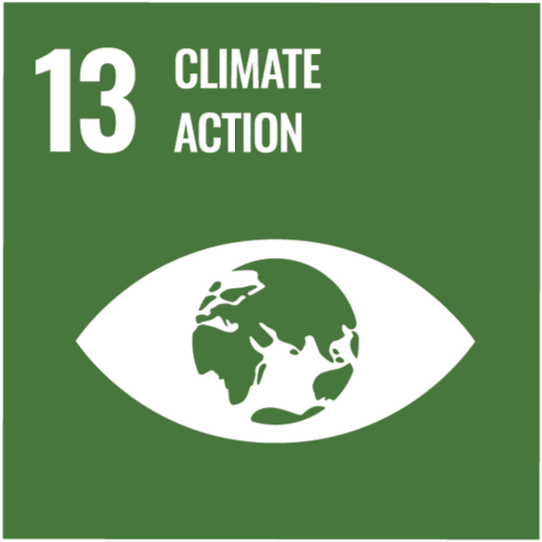
\includegraphics[width=.15\linewidth]{sdg13}
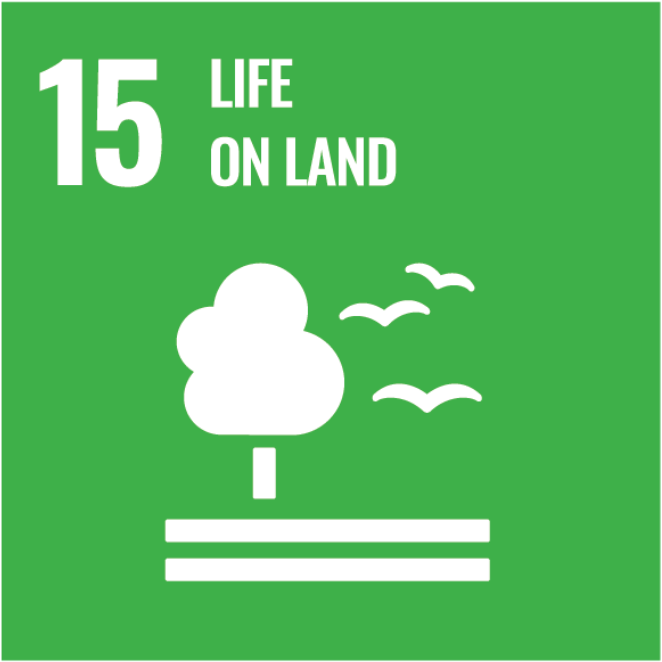
\includegraphics[width=.15\linewidth]{sdg15}
